\documentclass[a4paper,11pt]{scrartcl}

% packages
\usepackage[english]{babel}
\usepackage{graphicx}
\usepackage{url}
\usepackage{hyperref}
\usepackage{apacite} % keep after hyperref
\usepackage{tabularx}
\usepackage{fontspec}
    \setmainfont{Droid Serif}
    \setsansfont{Droid Sans}
    \setmonofont[SizeFeatures={Size=10}]{Droid Sans Mono}

% global options
\renewcommand{\baselinestretch}{1.2}
\pagestyle{headings}

% macro definitions
\newcommand{\imgref}[1]{{see \textit{figure \ref{#1}, page \pageref{#1}}}}
\newcommand{\imgrefplain}[1]{{\textit{figure \ref{#1}, page \pageref{#1}}}}
\newcommand{\tablerefplain}[1]{{\textit{table \ref{#1}, page \pageref{#1}}}}

\begin{document}

\author{Patrick P. Bucher and  Christopher J. Christensen}
\title{OAuth 2}
\subtitle{Computer Science Hot Topics}
\date{\today}
\maketitle

\section*{Abstract}

OAuth 2 is a delegation protocol that lives within the context of HTTP. It is mainly used to connect websites to one another and to secure APIs exposed to the web. OAuth 2 enables resource owners to delegate (limited) access to clients without sharing their credentials. OAuth 2 is neither an authentication nor an authorization protocol, but it defines the mechanisms to build such protocols. It does not define any cryptographic mechanisms, but leaves those decisions open for the implementation. The authorization server plays a key role in every web application that is secured through the means of OAuth 2. This paper gives an overview of the components and mechanisms involved in an OAuth 2 secured web application. Furthermore, a demo OAuth 2 application is presented as a case study to elucidate the role of and communication between different components involved in an OAuth 2 deployment. The JWT token format and common vulnerabilities of OAuth 2 are the subject of additional chapters.

\newpage

\tableofcontents
\newpage

\section{Introduction}

This section discusses what OAuth 2.0 is (henceforth OAuth 2, without the zero), and, especially, what it is not. Often times, OAuth 2 is perceived as some sort of security or authentication library that is capable of things way beyond its scope. Also, this section will mention what OAuth 2 is used for, how those ends were achieved before OAuth 2, and why OAuth 2 has gained traction. 

\subsection{The OAuth 2 Basics}

OAuth 2 is, simply put, a protocol that is used to authorize the access to protected resources. Since it works as a means to grant third-party applications limited access to these protected resources or HTTP services on behalf of a resource owner, it is often referred to as a delegation protocol \cite[p. 3]{oauth2-in-action}. If a user is shown the option to «login with Facebook» (or Google, or GitHub, etc.), OAuth 2 is probably being used.

\subsubsection{Roles}

The OAuth 2 protocol defines four roles that are listed below \cite{RFC6749}:

\begin{enumerate}
\item Resource Owner: Entity that grants access to protected resources.
\item Resource Server: Server that hosts the protected resources. Handles the requests to protected resources using access tokens.
\item Client: Application that sends requests to retrieve protected resources on behalf of the resource owner, once it has been granted authorization.
\item Authorization Server: Server that supplies access tokens to a client after the resource owner has been authenticated and has obtained authorization.
\end{enumerate}

\subsubsection{Access Token}
The access token can be viewed as the right to access a requested protected resource. This does not implicitly mean that the token will grant full access to all protected resources on a Resource Server. Often, or mostly, an access token only provides limited access to delegate specific actions by a resource owner \cite[p. 4]{oauth2-in-action}.

\subsubsection{Protocol Flow}

The flow of interactions between the OAuth 2 roles are as follows \cite[p. 5-6]{oauth2-in-action}:

\begin{enumerate}
\item An application (client) sends an authorization request directly to a resource owner, or, preferably, indirectly through an authorization server.
\item The client is authorized and receives a grant which represents the resource owner's authorization credentials.
\item The client can now request an access token from the authorization server with the freshly obtained grant.
\item The client is then authenticated by the authorization server once it has successfully validated the authorization grant. Then the authorization server creates and issues an access token.
\item The client can now request protected resources from the resource server with the access token.
\item If the access token has been successfully validated, the resource server provides the client with the requested resources.
\end{enumerate}

\subsection{The Dark Ages before OAuth 2}

Before OAuth 2, there were many alternatives to grant access to protected resources. Common approaches such as \textit{Credential Sharing}, \textit{Ask The User}, \textit{Universal Key} and \textit{Special Password} are explained briefly in this section. It is important to note that in none of these approaches an authorization server is used.

\begin{description}
    \item[Credential Sharing] This method copies a resource owner's credentials that are then replayed to the protected resource. It therefore requires the user to utilize the same credentials at the protected resource as at the client application. Since the user is exposing his credentials to the client application, the client is \textit{impersonating} the user. This leaves no way for the protected resource to tell if the user is requesting resources, or if the user is being impersonated. This can make sense if services and resources are offered by the same company, but causes tracability issues \cite[p. 7]{oauth2-in-action}.
    \item[Ask The User] The \textit{Ask The User} approach is a common practice despite the dangers that it poses. Until recently, Facebook asked new users for their credentials to their email account \cite{endgadget-facebook}, for example. This approach is used when credential sharing is not offered by the service holding a resource, and the client has no way to obtain the user's credentials across those different security domains. In this approach, the user is then asked for his username and password, which are then replayed on the protected resource \cite[p. 8]{oauth2-in-action}. The mechanism is similar to \textit{Credential Sharing}, but more transparent to the user.
    \item[Universal Key] A user can be given a universal key, which can be used to request protected resources directly. The problem is, that if this key is stolen, the resources are entirely and irrevocabely exposed. The universal key also does not work on a by-user basis, but globally for all users. This approach only makes sense between two trusted parties \cite[p. 10]{oauth2-in-action}.
    \item[Special Password] The special password in this case represents a password that is specifically created solemnly on the side of the protected resource for sharing with third-party-services. This means the user need not share his credentials with the third-party services. Although this is a more desirable approach, the user is now required to keep track of yet another password \cite[p. 10]{oauth2-in-action}.
\end{description}

\subsection{The Attraction of OAuth 2}

The insecure and unsatisfactory approaches mentioned before, even though possibly still in wide use, are all obsolete nowadays. OAuth 2 is a solution that lets users grant limited and fine-grained access to their protected resources separately for different clients. This approach requires an authorization server: a system that is trusted by the protected resource and the resource owner alike. The authorization server is aware of all the granted rights and issues special-purpose security credentials for client access of a specified scope: access tokens. No credentials are shared in the process \cite[p. 11]{oauth2-in-action}.

An authorization server might require clients to authenticate themselves, so that only authorized clients can retrieve grants for protected resources. (This looks similar to the \textit{Universal Key} approach, but here the pre-shared secret key is not used for the resource access, which only works with a valid access token, but only for the authentication of the client itself.) Another similarity to the approaches discussed before is that OAuth 2 does not require the user being present when resources are accessed on his behalf \cite[p. 14]{oauth2-in-action}.

Having protected resources being accessed without the user's presence might sound intransparent, but one must remember that the user gave his consensus for the access delegation earlier in the process. Therefore it is important that clients state their request access scopes correctly and transparently. This approach is often referred to as \textit{TOFU: Trust On First Use} \cite[p. 15]{oauth2-in-action}.

\subsubsection{The Limitations of OAuth 2}

Even though OAuth 2 solves the delegation problem well, it is no silver bullet.

\begin{itemize}
    \item OAuth 2 is neither an authentication nor an authorization protocol, it is just a framework to base those kinds of protocols onto.
    \item The authorization server plays a key role in every OAuth 2 deployment and thus bears the risk of being the single point of failure for security breaches.
    \item OAuth 2 lives in the context of HTTP and requires secured connections (TLS) to be of any real use.
    \item Delegating access to other users (as opposed to clients) is not provided by OAuth 2. However, this can be implemented using the UMA (User Managed Access) protocol, an OAuth 2 extension.
    \item Both the protected resource and the authorization server need to understand the token format. (On the plus side, the client does not need to.)
\end{itemize}

Most of these shortcomings are limitations in the scope of the protocol definition, and are addressed by additional protocols and standards, some of them are OAuth 2 extensions. The key role the authorization server plays bears a high risk. It is easier though to secure one critical system well than to secure a multitude of systems equally sufficient \cite[p. 18-20]{oauth2-in-action}.

\vskip 13pt

The next chapter goes into more detail on the components in OAuth 2, and how they interact with one another in a process called the \textit{Authorization Grant}, the most common OAuth 2 process.

\newpage

\section{Case Study: Gossip Server}

A practical example is often useful to gain a better understanding of a process requiring different actors and multiple steps. The simple \textit{Gossip Application}, which can be found on GitHub (\url{https://github.com/patrickbucher/oauth2-demo}, with further information on how to run the applications and how to play with it), demonstrates the OAuth 2 authorization grant flow with three web applications written in Go:

\begin{description}
    \item The \textit{client}, which offers a web interface to retrieve gossip from a backend application. 
    \item The \textit{resource}, which offers a REST endpoint that provides gossip to authorized clients and users.
    \item The \textit{authserver}, which lets the client authorize itself to get access tokens, and validates access tokens for the resource before any gossip is delivered to the client.
\end{description}

The \textit{client} has a \texttt{client\_id} with a \texttt{client\_secret} (pre-shared between \textit{authserver} and \textit{client}), so that the \textit{client} can authenticate against the \textit{authserver}. The \textit{client} does not know the \textit{authserver}, it just knows how to authenticate towards \textit{any} authorization server: with its credentials, that is.

The \textit{resource owner} has its own gossip stored on the \textit{resource} server, and wants to access it through the \textit{client}. The \textit{resource owner} is neither aware of the \textit{resource server}, nor of the \textit{authserver}, but knows how to access the \textit{client}.

The \textit{resource} server knows the coordinates of the \textit{authserver}, and also knows that any request to its resources (the gossip) must be authorized using an access token, which must be verified against the \textit{authserver}.

\subsection{OAuth 2 Authorization Grant: A Conversation}

Even though the great Dijkstra frowned at antropomorphisms in computer science \cite{EWD936}, seeing the components of a system as human-like actors can often help gaining clarity. It is true that those actors do not «want» or «dismiss» anything on their own, it is the programmer's intention which is codified in those components. And the programmer needs to take different points of view when developing or understanding those components, and be aware of what components «knows» what and when.

A possible conversation between the actors of an OAuth 2 grant process -- the \textit{resource owner}, the \textit{client}, the \textit{authorisation server}, and the \textit{protected resource} -- might look as follows (the process can be followed along on \imgrefplain{fig:auth-grant}).

\begin{figure}
    \centering
    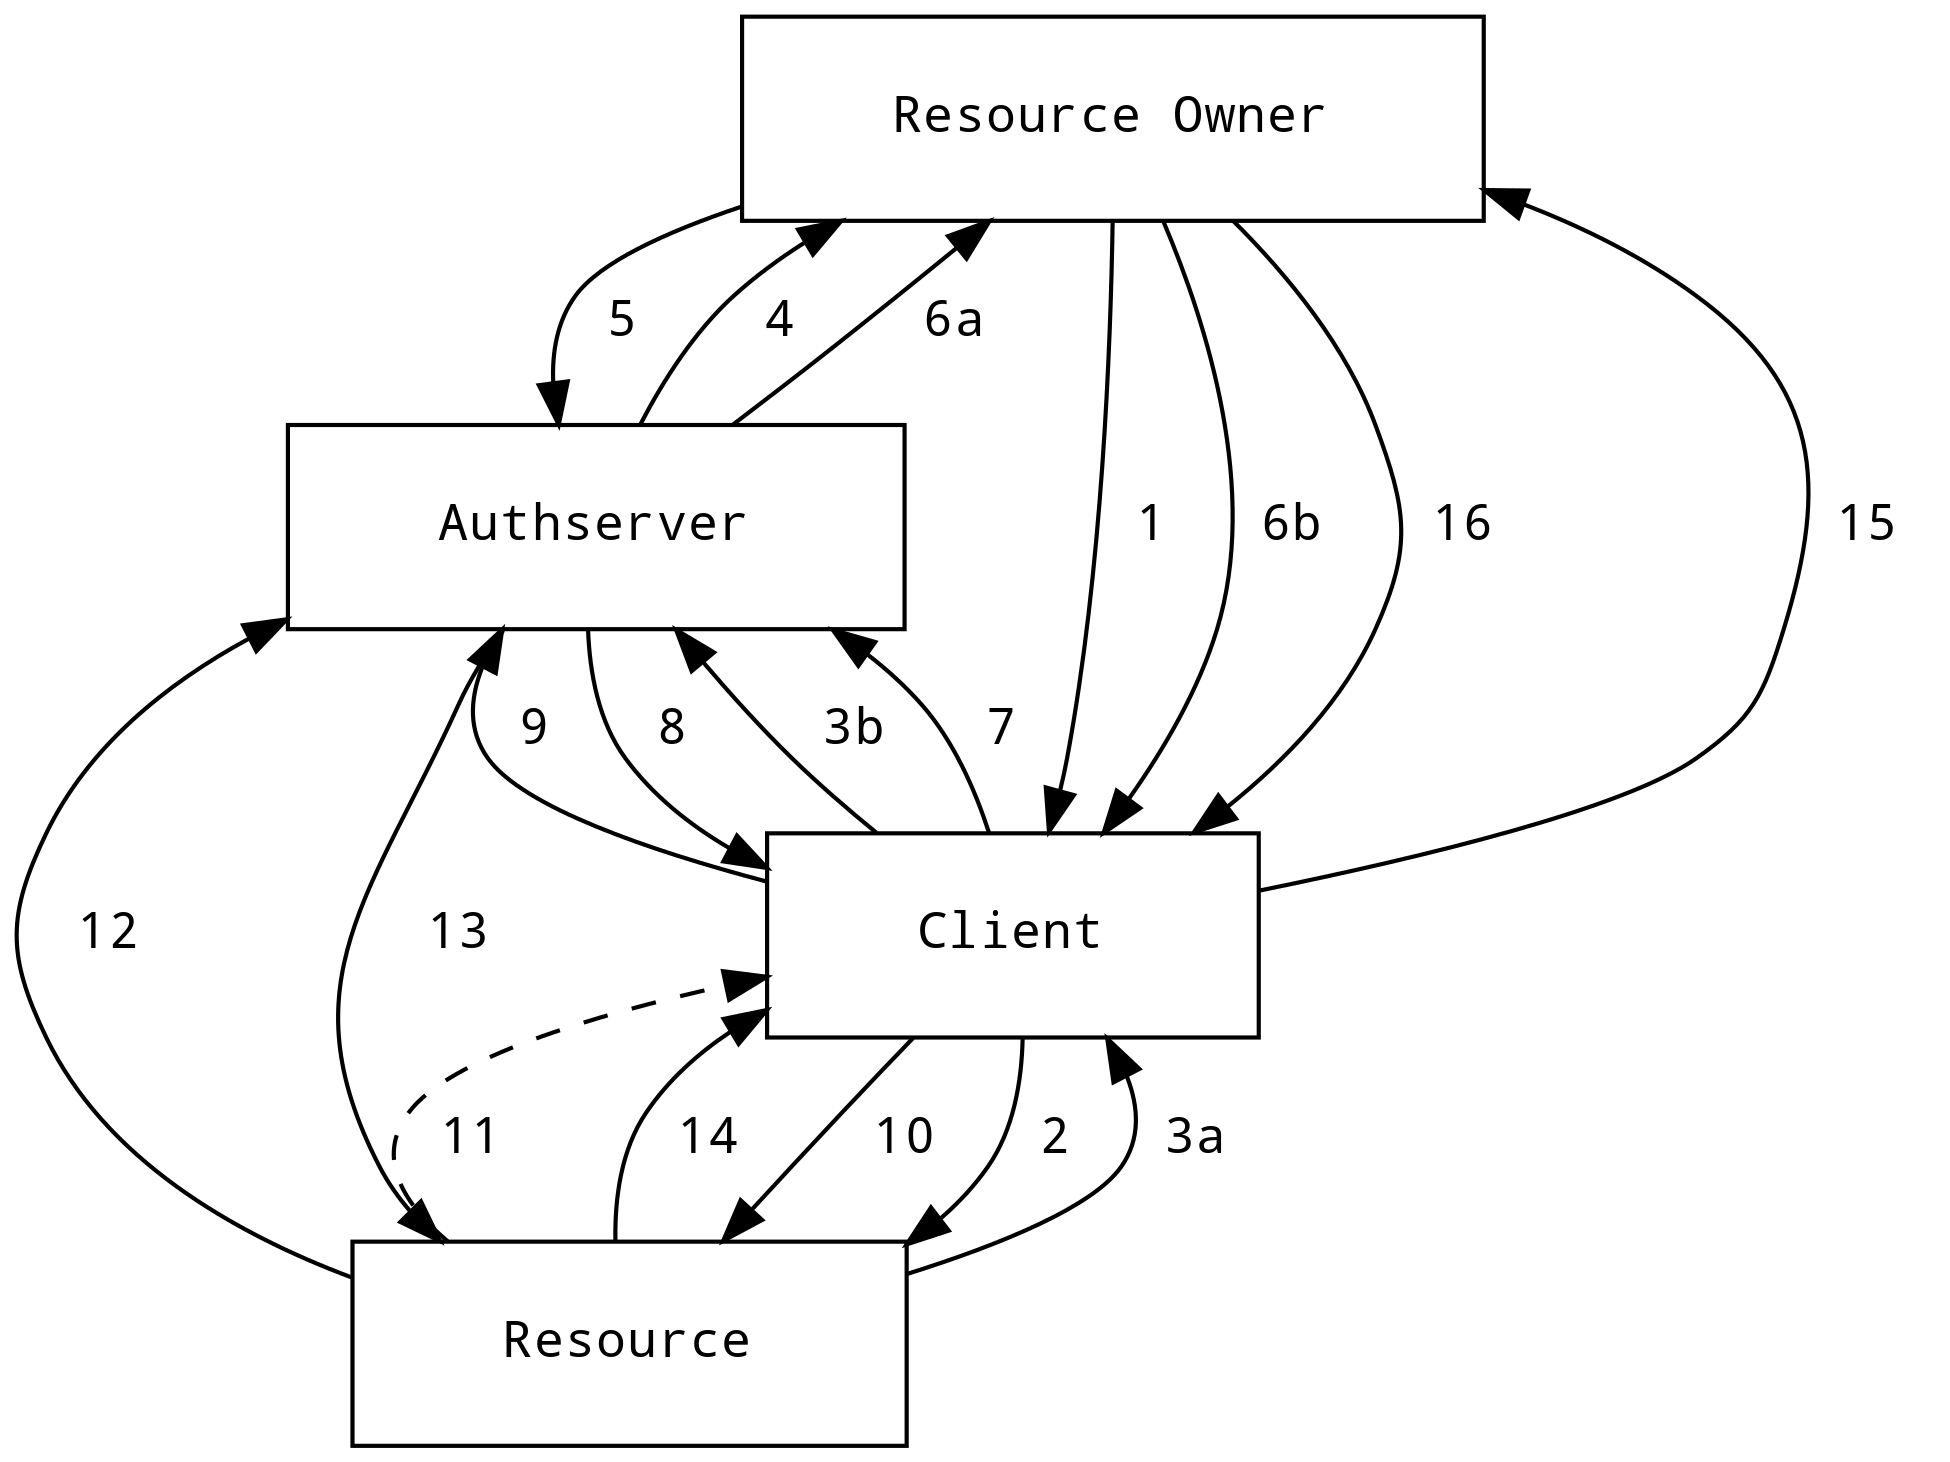
\includegraphics[width=\linewidth]{auth-grant.png}
    \caption{The OAuth 2 Authorization Grant}
    \label{fig:auth-grant}
\end{figure}

\subsubsection{Act I: Getting a Token}

In the first act, the protagonists are negotiating the access rights of a \textit{resource owner} delegated to the \textit{client}. The result of this process is the \texttt{access\_token}, which is an artifact representing the granted access right.

\begin{description}
    \item \texttt{1} \textbf{Resource Owner to Client} I have some gossip stored on the \textit{resource} server. Please retrieve that gossip for me, you can tell the \textit{resource} server that my name is «Joe».
    \item \texttt{2} \textbf{Client to Resource} Joe asked me to retrieve his gossip for him. Could you please hand me that over? I leave my coordinates, and a \texttt{state} identifier, just in case…
    \item \texttt{3a} \textbf{Resource to Client} Really? How can I be sure that it's really Joe asking for his gossip? If it really were Joe to ask me for the gossip, you'd bring along some \texttt{access\_token} to prove that Joe issued the request. Anybody could ask me to hand over Joe's gossip, but nobody but Joe has the rights to access it. I don't even know if you are trustworthy at all. You first must prove it! So here's the deal: Take this address, it belongs to the \textit{authserver}. I'm going to send it to Joe -- or whoever is using you at the moment… if somebody is actually using you! Joe has to identify himself with his username and password, and in the same step tell the \textit{authserver} that you are a trustworthy client. I'm writing down the coordinates of your \texttt{/callback} endpoint you told me about, so that the \textit{authserver} can come back to you after Joe authorized you, and I make sure the \textit{authserver} gets that note when I'm redirecting Joe to it. I'll also forward your \texttt{state} identifier, so you can remember this request later. OK, see you later… maybe.
    \item \texttt{3b} \textbf{Client} OK, let me… Wow! What is happening? The resource owner is getting forwarded away from me!
    \item \texttt{4} \textbf{Authserver to Resource Owner} Hi there, I'm the \textit{authserver}. Remember me? You probably registered here and even verified your email address some time ago. The protected \textit{resource} sent you here, because some \textit{client} tried to access your resources on your behalf. I don't know if that's fine for you. If you really requested the \textit{client} to get the protected resource for you, then please tell me your username and password. When you do that, you automatically authorize the \textit{client} to get your resources.
    \item \texttt{5} \textbf{Resource Owner to Authserver} Hey, of course I remember you. I use you now and then to login to web sites that trust you. So my username is «Joe» and my password is… \textit{[unintelligible]}. It really was me who asked the \textit{client} to fetch the resource for me, so you can trust it.
    \item \texttt{6a} \textbf{Authserver to Resource Owner} Hey Joe, I found your account, and the password you entered matches what is stored in my credentials store. I'm writing down that you trust the \textit{client} from now on. The \textit{resource} (we trust each other) gave me a note on how to send you back to the client, which I'm going to do now. Here's also an \texttt{auth\_code} the \textit{client} can use once to get an \texttt{access\_token} for you. Goodbye Joe! See you again once your token is expired!
    \item \texttt{6b} \textbf{Resource Owner} OK, it looks like there's a forward going on again…
    \item \texttt{7} \textbf{Client to Authserver} Wow, I just got called back from you! The \textit{resource} told me that this is going to happen! Glad to hear that Joe trusts me. (It's not that much of a surprise, actually, because he told me already that I should fetch his resource.) And I remember that \texttt{state} identifier, it belongs to the initial request Joe let me do. Thanks also for your coordinates and the \texttt{auth\_code}. I'm going to use them right away to fetch an \texttt{access\_token} from you. By the way: We already know each other. I once registered with my \texttt{client\_id}, and you gave me this \texttt{client\_secret} you hopefully still remember! Let me send those to you base64 encoded as a HTTP basic \texttt{Authorization} header. OK, can I please get an \texttt{access\_token} for Joe?
    \item \texttt{8} \textbf{Authserver to Client} Hello again, thanks for calling my \texttt{/token} endpoint. Let's see… Indeed, I remember the \texttt{client\_id} and \texttt{client\_secret} you sent to me, all so nicely and securely wrapped up in the \texttt{Authorization} header. And this is really the \texttt{auth\_code} I just sent you before. And it belongs to Joe. And Joe authorized you as a client. The \texttt{auth\_code} is a one-time password, so let's forget about it once you got the \texttt{access\_\-token}, all right? So here's your \texttt{access\_token}, I'm going to remember it. Now hurry up, this token is going to expire soon! And we don't want Joe to go through all this hassle again, do we?
    \item 9 \textbf{Client to Authserver} Great, thanks! I'm going to replay Joe's initial request right away, but this time I'll attach that token you've given me to the \textit{resource} in the \texttt{Authorization} header. See you later, maybe…
\end{description}

\subsubsection{Act II: Using a Token}

Once an \texttt{access\_token} is granted, it can be used to retrieve resources. The second act can be replayed many times, as long as the \texttt{access\_token} is valid.

\begin{description}
    \item \texttt{10} \textbf{Client to Resource} So, here's Joe's initial request again, but this time, I also got this nice \texttt{access\_token} with me. So open up and hand me over Joe's gossip! (He really is on a mission and wants to spread it…)
    \item \texttt{11} \textbf{Resource to Client} OK, now this is an \texttt{access\_token}? I don't know, but the \textit{authserver} does! Hang on, I quickly double check, if that is valid.
    \item \texttt{12} \textbf{Resource to Authserver} Hey, it's me, I've just redirected some \textit{client} to you a couple of seconds ago. I remember that he wanted to get Joe's resources. He gave me this \texttt{access\_token}. Is that thing valid?
    \item \texttt{13} \textbf{Authserver to Resource} Hello, my dear old friend! Let's see: Indeed, I issued such an \texttt{access\_\-token}, and it was only seconds ago. So the token is still valid. And I remember that I issued it for Joe's scope. Perfectly fine with me, go ahead and hand over Joe's resource to that \textit{client}!
    \item \texttt{14} \textbf{Resource to Client} Are you still there? OK, great! I have good news for you! The \texttt{access\_token} you sent to me is valid! So here's Joe's gossip! You can come back later to me. I'll always check that token against the \textit{authserver}, because only he knows all the security details. (I just know some gossip.)
    \item \texttt{15} \textbf{Client to Resource Owner} Hey Joe, here I am again! And I got your gossip with me. I'm going to display it as a HTML page. When you access it anytime soon, you're not required to authenticate yourself and authorize me again, because me, the \textit{authserver}, and the \textit{resource} managed to sort that out for you. But if you wait for too long, we might need to go through that whole process again. I'm so happy that we are all compiled programs that do just execute and not think too much…
    \item \texttt{16} \textbf{Resource Owner to Client} Hey, thanks for all that work! I'm now going to enjoy my gossip. See you later!
\end{description}

\newpage

\section{JSON Web Tokens (JWT)}

This chapter is mainly about structured JSON Web Tokens. However, there will also be a brief look throughout the chapter at what a token can be, and what other token implementations exist. All code examples are in JavaScript.

\subsection{OAuth 2 Tokens}

Since nothing works without them, tokens are viewed as the centerpiece of OAuth. A client requests a token from the authentication and authorization server (henceforth «auth server») and passes it on to the protected resource. The protected resource validates it and verifies if the attached permissions and rights allow the client to proceed with its request. The tokens can be seen as the result of the delegation act.

It is important to note that OAuth 2 does not define what a token is, thus leaving the implementation to each deployment. OAuth 2 can therefore be used in many different deployments with varying requirements. This is one of the reasons OAuth 2 is chosen over other protocols such as SAML or Kerberos.

Upon receiving a token, the client must merely send the token along with its request. This means that the client does not need to know anything about what a token is or how it is implemented. The only thing the client needs to know, is how to obtain and use it. Both the auth server and protected resource need to know more about it, though. The auth server must know how to create one, whereas the resource owner needs to know how to recognize and validate it.

\subsection{Overview of OAuth 2 Token Implementations}

Since OAuth 2 does not dictate the form of its tokens, there are many different implementations. 

One approach would be to generate a random string which is then stored in a database. This random string represents the token. Upon receiving the token, the resource owner looks the string up in this database and retrieves additional information about a client's or user's permission and rights. The downside of this approach is that the auth server and resource owner both need to have access to a shared database. This is not always adviseable nor possible. (Another option is that the protected resource verifies the token at the auth server, as it was done in the case study in the chapter before.)

What will be looked at closer in this chapter is the implementation of structured tokens. In this case, tokens carry information, which the protected resource can parse and use for validation. An extension of this approach would be the use of token introspection, although this will not be the subject here, because it does not really further enhance the basic understanding of tokens in itself.

\subsection{Structured Tokens: JSON Web Tokens (JWT)}

According to the IETF «JSON Web Token (JWT) is a compact, URL-safe means of representing claims to be transferred between two parties» \cite[p. 1]{RFC7519}. It carries all the information necessary in itself to grant the client or the user access to a protected resource. It thus enables indirect communication between the auth server and resource owner without further API calls. The information that the JWT carries could be for instance an expiration time\-stamp or information about the user who gave authorization to it. Although JWT does allow for any keys and values to be placed into its JSON objects, they do set a guideline with a few standard claims to avoid key clashing between different implementations. These claims can be seen in \tablerefplain{tbl:jwt-claims} \cite[p. 185]{oauth2-in-action}.

\begin{table}
    \begin{tabularx}{\linewidth}{l | X}
        \textbf{Claim Name} & \textbf{Claim Description} \\
        \hline
        \texttt{iss} & The \textit{issuer} of the token. This is an indicator of \textit{who created this token}, and in many OAuth 2 deployments this is the URL of the auth server. This claim is a single string. \\
        \texttt{sub} & The \textit{subject} of the token. This is an indicator of \textit{who the token is about}, and in many OAuth 2 deployments this is a unique identifier for the resource owner. In most cases, the subject needs to be unique only within the scope of the issuer. This claim is a single string. \\
        \texttt{aud} & The \textit{audience} of the token. This is an indicator of \textit{who is supposed to accept the token}, and in many OAuth 2 deployments this includes the URI of the protected resource or protected resources that the token can be sent to. This claim can be either an array of strings or, if there's only one value, a single string with no array wrapping it. \\
        \texttt{exp} & The \textit{expiration} time\-stamp of the token. This is an indicator of \textit{when the token will expire}, for deployments where the token will expire on its own. This claim is an integer of the number of seconds since the UNIX Epoch, midnight on January 1, 1970, in the Greenwich Mean Time (GMT) time zone. \\
        \texttt{nbf} & The \textit{not-before} time\-stamp of the token. This is an indicator of \textit{when the token will begin to be valid}, for deployments where the token could be issued before it becomes valid. This claim is an integer of the number of seconds since the UNIX Epoch, midnight on January 1, 1970, in the GMT time zone. \\
        \texttt{iat} & The \textit{issued-at} time\-stamp of the token. This is an indicator of \textit{when the token was created}, and is commonly the system time\-stamp of the issuer at the time of token creation. This claim is an integer of the number of seconds since the UNIX Epoch, midnight on January 1, 1970, in the GMT time zone. \\
        \texttt{jti} & The \textit{unique identifier} of the token. This is a value \textit{unique to  each token created by the issuer}, and it is often a cryptographically random value in order to prevent collisions. This value is also useful for preventing token guessing and replay attacks by adding a component of randomized entropy to the structured token what would not be available to an attacker.
    \end{tabularx}
    \caption{Standard JSON Web Token Claims\label{tbl:jwt-claims}}
\end{table}

The JSON Web Token is, as its name implicates, a JSON object, which gets encapsuled into a suitable format for transmission over, for instance, HTTP. There are two main distinctions between different types of JWTs: unsigned and signed tokens.

\subsubsection{Unsigned JSON Web Tokens}

The unsigned JWT consists of two parts that are separated through a period. The first part represents the header, which contains information about the type of the token, and other information the resource owner needs to know about the token itself. In its JSON form before encoding, it could look as follows:

\begin{verbatim}
{
  "typ": "JWT",
  "alg": "none"
}
\end{verbatim}

The second part of the token is called payload. The payload carries all data that the protected resource needs to validate and verify a request from the client. 

\begin{verbatim}
var payload = {
  iss: 'http://localhost:9001/',
  sub: code.user ? code.user.sub : undefined,
  aud: 'http://localhost:9002/',
  iat: Math.floor(Date.now() / 1000),
  exp: Math.floor(Date.now() / 1000) + (5 * 60), // five minutes
  jti: randomstring.generate(8)
};
\end{verbatim}

To create an unsigned JWT, one merely needs to create a header and payload, serialize the JSON objects as strings, and then encode the two strings using base64 URL encoding. These two strings made out of header and payload are then concatenated via a period followed by a period at the end. An unsigned JWT could look something like this:

\begin{verbatim}
eyJ0eXAiOiJKV1QiLCJhbGciOiJub25lIn0.eyJzdWIiOiIxMjM0NTY3ODkwIiwib
  mFtZSI6IkpvaG4gRG9lIiwiYWRtaW4iOnRydWV9.
\end{verbatim}

The downside of an unsigned JWT is obviously that it has no encryption, so that any client can dissect, analyse and then create its own tokens. They are therefore considered unsafe.

\subsubsection{Signed JSON Web Tokens}

Signed JWTs are encrypted before transmission and are therefore safer than unsigned tokens. Signed JWTs have a third part that is again concatenated with the header and payload at the end of the token. This third part holds information about how the token was encrypted. JWT has created a suite of useful specifications called JSON Object Signing and Encryption standards, or JOSE in short, to help with the encryption of these tokens. It covers various topics such as encryption, signatures and key storage formats.

There are many ways of creating signed JWTs. There are also two main signing types: asymmetric and symmetric signing. Symmetric signing uses a shared secret between the auth server and protected resource. The token could then be encrypted using HS256. The header would then look something like the code below:

\begin{verbatim}
var header = { 'typ': 'JWT', 'alg': 'HS256'};
\end{verbatim}

The header and payload are then encrypted as shown in the next code example.

\begin{verbatim}
var access_token = jose.jws.JWS.sign(header.alg,
   JSON.stringify(header),
   JSON.stringify(payload),
   new Buffer(sharedTokenSecret).toString('hex'));
\end{verbatim}

The token then looks something like this:

\begin{verbatim}
eyJ0eXAiOiJKV1QiLCJhbGciOiJIUzI1NiJ9.eyJpc3MiOiJodHRwOi8vbG9jYW
  xob3N0OjkwMDEvIiwic3ViIjoiOVhFMy1KSTM0LTAwMTMyQSIsImF1ZCI6Imh
  0dHA6Ly9sb2NhbGhvc3Q6OTAwMi8iLCJpYXQiOjE0NjcyNTEwNzMsImV4cCI6
  MTQ2NzI1MTM3MywianRpIjoiaEZLUUpSNmUifQ.WqRsY03pYwuJTx-9pDQXft
  kcj7YbRn95o-16NHrVugg
\end{verbatim}

The problem with symmetrical approaches is that the auth server and protected resource have to be tied closely to be able to share a secret. If this is not the case, then the asymmetrical approach may be more suitable. Here the auth server has a private and a public key, which it uses to create the tokens. The protected resource must have access to the auth server's public key in order to verify the token. One possible way to sign such a token would be with the RS256 signature method by JOSE. The header would then look as follows:

\begin{verbatim}
var header = { 'typ': 'JWT', 'alg': rsaKey.alg, 'kid': rsaKey.kid };
\end{verbatim}

The access token is then created like this:

\begin{verbatim}
var access_token = jose.jws.JWS.sign(header.alg,
   JSON.stringify(header),
   JSON.stringify(payload),
   privateKey);
\end{verbatim}

This method generates much longer tokens. To mitigate this, token introspection is used, where the public key information of the auth server is hosted on a known URL, so that the protected resource can fetch it when needed.

\subsubsection{Validating JSON Web Tokens: 3 Examples}

Here are three ways the protected resource could validate a received token from the client. The first example is implemented with an unsigned token. The second example with a signed symmetrical token, and the third with an signed asymmetrical token.

\paragraph{Example 1: Validation of Unsigned Token}

\begin{verbatim}
// 1. Decode Base64URL and parse JSON
var tokenParts = inToken.split('.');
var payload = JSON.parse(base64url.decode(tokenParts[1]));

// 2. Validate
if (payload.iss == 'http://localhost:9001/') {
  if ((Array.isArray(payload.aud) &&
       __.contains(payload.aud, 'http://localhost:9002/')) ||
       payload.aud == 'http://localhost:9002/') {
    var now = Math.floor(Date.now() / 1000);
    if (payload.iat <= now) {
        if (payload.exp >= now) {
            req.access_token = payload;
        }
    }
  }
}
\end{verbatim}

\paragraph{Example 2: Validation of Signed Symmetric Token}

\begin{verbatim}
// 1. Get shared secret
var sharedTokenSecret = 'shared OAuth token secret!';

// 2. Decode and parse token
var tokenParts = inToken.split('.');
var header = JSON.parse(base64url.decode(tokenParts[0]));
var payload = JSON.parse(base64url.decode(tokenParts[1]));

// 3. Validate
if (jose.jws.JWS.verify(inToken,
    new Buffer(sharedTokenSecret).toString('hex'), 
    [header.alg])) {
    
    // All previous validation from example 1 go here...
}
\end{verbatim}

\paragraph{Example 3: Validation of Signed Asymmetric Token}

\begin{verbatim}
// 1. Get public key of auth server
var publicKey = jose.KEYUTIL.getKey(rsaKey);

// 2. Validate
if (jose.jws.JWS.verify(inToken,
    publicKey,
    [header.alg])) {

    // All previous validation from example 1 go here...
}
\end{verbatim}

\subsection{OAuth 2 Token Lifecycle}

There are many ways to define the lifecycle of a token. JWTs are stateless and provide access tokens that expire, but also provide refresh tokens (that also expire after a longer period of time), but they cannot be revoked. Other specifications use token revocation, where the client requests for the token to be deleted and thus closes the token lifecycle. OAuth 2 defines a token revocation protocol.

\newpage

\section{OAuth 2 Vulnerabilities}

OAuth 2 does not guarantee security, since it does not define any implementations. Even though OAuth 2 can be seen as a solid security protocol, vulnerabilities can arise when implementing it in insecure manners. This chapter is about a few chosen vulnerabilities on each parties side.

\subsection{Client Vulnerabilities}

Even though an OAuth 2 client does not hold the application's data or store any user credentials, an authorized and trusted client is both a rewarding and a vulnerable target for an attacker. It carries senstivie data (authorization codes, access tokens), and the user's trust relationship to the client can easily be exploited, if the client is not implemented properly.

\subsubsection{Secret Theft}

Whenever a client needs to manage a secret — authorization codes, access and refresh tokens in the case of OAuth 2 — it can be stolen and misused. In this case, it can lead to theft of information from the protected resource, or worse, manipulation of the protected resources. This makes it a necessity to store these secrets at a place where outside parties will not be able to access them. Secrets also must not be written to log files.

\subsubsection{CSRF Attacks}

Cross-Site Request Forgery (CSRF) is when malicious applications make clients execute undesired actions via a website for which a user is authenticated. The malicious application tricks the user or the browser being used into sending a request to perform a task on a URI. Although the malicious application intended the request, it was the authenticated user that made it. The malicious code is usually embedded in HTML or JavaScript code on a website or in an email message. Upon action of the user, the code is executed without the user knowing. A plausible list of events would be the following:

\begin{enumerate}
  \item The victim requests a page from the attacker's server.
  \item The attacker's server responds with HTML containing malicious code pointing to a task URL on the resource owner's server.
  \item The victim's browser loads the URL that sends cookies to the resource owner.
  \item The resource owner authenticates the victim.
  \item Loading the task URL triggers an action at the resource owner.
  \item The attacker forges the authorization code of the authorization server.
  \item The attacker sends a CSRF attack to the client at the client's redirect URI (with the authorization code).
  \item The victim's browser loads the redirect URI with the authorization code.
  \item The client sends the authorization code to the authorization server.
\end{enumerate}

One of the most effective ways to mitigate such an attack is to add a random state parameter, as it is demonstrated in the case study. This parameter is passed to the authorization server on its first request. The authentication server must return this state parameter upon which the client can compare if it still matches. If not, the client can terminate the process.

\subsection{Protected Resource Vulnerabilities}

Attacking the protected resource of an OAuth 2 deployment is the most obvious choice, for this component offers the applications main assets: the user's data.

\subsubsection{Token Leak}

If a token is leaked to an attacker via hijacking or due to weak entropy or overly wide scopes, the resource owner could give the attacker access to protected resources.

\subsubsection{Cross-Site Scripting (XSS)}

An attacker can trick a victim into following a forged URI containing an XSS attack. This attack is quite common and is listed in the OWASP Top Ten \cite{owasp2017}. The protected resource becomes vulnerable when the API endpoints have been weakly designed or not properly implemented. Without cleansing user inputs, for example, the attacker could add malicious code into the query string of a URI that hits an API endpoint, and then execute the malicious code upon response. In this example, JavaScript code is injected where a language code (\texttt{de}, \texttt{en}, etc.) is expected. 

\begin{verbatim}
http://localhost:9002/endpoint?access_token=TOKEN
    &language=<script>alert('XSS')</script>
\end{verbatim}

The endpoint is poorly implemented, processes the request, and the pretended language code (i.e. the malicious JavaScript code) is executed. Tokens, which are held in the browser session, thus can be accessed from the malicious code and be sent to the attacker over an AJAX request.

\subsection{Authorization Server Vulnerabilities}

The authorization server is the most complex entity in a OAuth 2 deployment, and therefore also has the most possible pitfalls. It both has a user-facing interface (authorization/authentication page for front-channel communication) and a machine-facing interface (API for back-channel communication). In addition to general web security advice (use TLS, secure the server and logs, etc.), some special advice specific to OAuth 2 is given here to avoid common vulnerabilities.

\subsubsection{Session Hijacking}

An authorization code, as it is used in the case study, is a one-time password, and therefore must only be allowed to be used exactly once. Since the authorization code is sent back to the client by the means of a redirect, this one-time password stays in the browser history, even if the user logs out off the client and/or the authorization server. An attacker with access to the same computer (and to the browser history) could therefore tamper this original redirect request to get a fresh \texttt{access\_token} and, thus, access to the original user's scope.

The OAuth 2 specification gives clear advice on how to prevent such attacks: An authorization code must only be used once, and then must be invalidated by the authorization server. Optionally, all the access tokens issued with an authorization code can be revoked upon a second attempt to use it \cite[section 4.1.3]{RFC6749}.

\subsubsection{Redirect URI Manipulation}

The \texttt{redirect\_uri} a client uses to get the authorization code sent to must be initially registered at the authorization server. The authorization server then must check on every request that the \texttt{redirect\_uri} actually used \textit{matches} the \texttt{redirect\_uri} initially registered. However, this matching can be done in different ways:

\begin{enumerate}
    \item Exact matching: check for equality.
    \item Allowing subdirectory: the path of the actual \texttt{redirect\_uri} can contain additional elements to the registered value.
    \item Allowing subdomain: any subdomain on the registered host can be used with the same path.
    \item Allowing both subdirectory and subdomain: a combination of the latter two options.
\end{enumerate}

Option 1, exact matching, is the safest option. The other options are unsafe and can be exploited, especially in a cloud hosting setting. A user of service \url{foo.cloudhosting.com} could be redirected to the attacker's service hosted on the same environment, say \url{bar.cloudhosting.com}, if a different subdomain is allowed. If a different path (subdirectory) is allowed, the attacker can achieve the same by using relative paths (\texttt{../../..}). If a user can be sent to such a forged page, his authorization code will be redirected to the attacker, giving him access to the user's authorized scope.

\newpage 

\section{Conclusion}

OAuth 2 is currently the de facto standard to secure web applications. Even though the OAuth 2 core specification does not provide a bullet-proof recipe for building safe web applications, it is a good starting point, for there is a huge ecosystem consisting of supplementary protocols, techniques, libraries, frameworks, books, articles, best practices and ready to use components. One of the strengths of OAuth 2 is actually that is does \textit{not} prescribe or define implementation details such as cryptographic algorithms, which might be subject to change as time goes. Like an organism that lives longer than its cells, OAuth 2 might be still around after its current building blocks have been deprecated.

The case study shows that a simple OAuth 2 deployment can be implemented with off-the-shelf programming tools. A good HTTP library (for both client and server) combined with some basic crypto functionality is all it needs, even though it is highly recommended to use higher-level abstractions or ready-made components when implementing productive applications. (Some techniques applied in the case study are clear security red flags, such as storing passwords in cleartext, or communicating over plain HTTP.) Since the focus of the example code is only on the communication flow, the case study still makes a point: A simple web application can be sufficiently secured with OAuth 2 using simple tools, even though it takes some effort to understand the intricacies of each and every step.

Unlike the case study, real-world applications do not use opaque random strings as tokens, but encode the delegated access rights into a cryptographically secured token format called JWT. This common token format not only makes it easier to implement OAuth 2 applications (thanks to well-tested and convenient libraries), but also helps to decouple the protected resource from the authorization server. (In the case study, the protected resource still relied on the authorization server to validate tokens.)

Since OAuth 2 lives in the context of the modern web, it is subject to common security vulnerabilities such as session hijacking and cross-site scripting. Common vulnerabilities have common, time-proofed and well understood mitigations, and the OAuth 2 specification and its related documents offer good advice on how to harden web applications against those threats.

As the web becomes the most common way of deploying applications, more sensitive data is moved into web applications, and as OAuth 2 stays the state of the art standard for securing web applications, a solid understanding of OAuth 2 is a necessity for professional web developers nowadays.

\newpage

\bibliographystyle{apacite}
\bibliography{paper}
\listoffigures
\addcontentsline{toc}{section}{List of Figures}
\listoftables
\addcontentsline{toc}{section}{List of Tables}

\end{document}
